
\documentclass{article}

\usepackage{a4wide,tikz}
\usetikzlibrary{mindmap,trees}
\newcommand{\mtex}{{\Huge \bf{\color{red}M}TEX\,}}%
\usepackage[margin=0pt,hmargin={-0.5cm,0cm},papersize={10.35cm,9.26cm}]{geometry} 
\begin{document}
\pagestyle{empty}


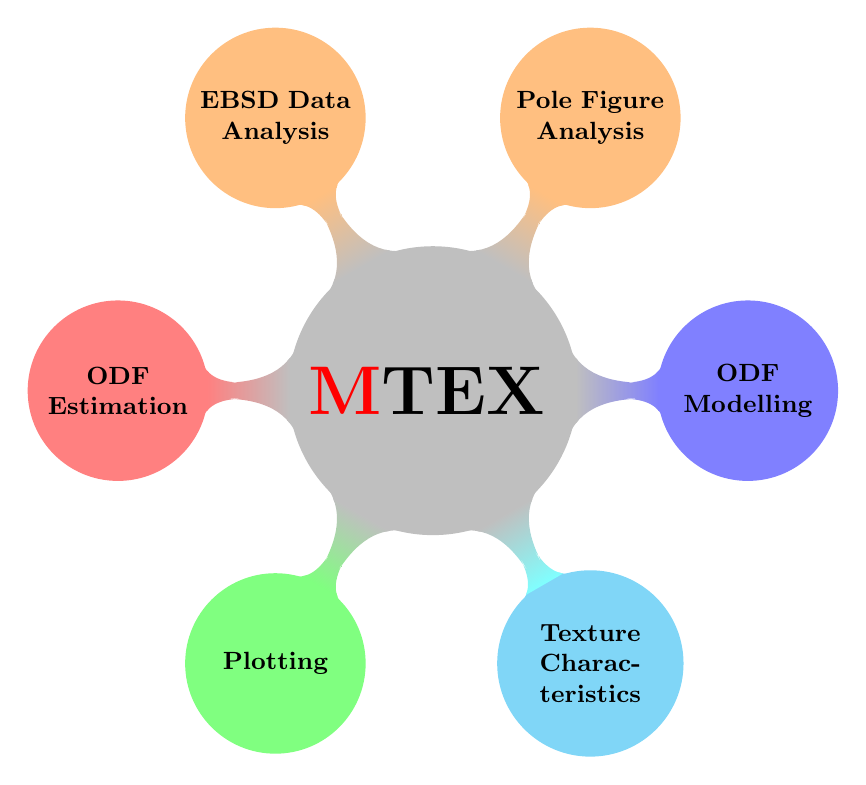
\begin{tikzpicture}[scale = 1]
  \definecolor{myblue}{HTML}{92dcec}

  \path[mindmap, minimum size=2cm, concept color=gray!50!]
  node[concept] {\mtex} 
  child[grow = 0, concept color=blue!50] 
  { node at (0:-1) [concept] {\bf ODF Modelling}}
  child[grow = 60, concept color=orange!50] 
  { node at (60:-1)[concept](pf) {\bf Pole Figure Analysis}}
  child[grow = 120, concept color=orange!50] 
  { node  at (120:-1) [concept](pf) {\bf EBSD Data Analysis}}
  child[grow = 180, concept color=red!50] 
  { node at (180:-1)[concept](pf) {\bf ODF Estimation}}
  child[grow = 240, concept color=green!50] 
  { node at (240:-1) [concept](pf) {\bf Plotting}}
  child[grow = 300, concept color=cyan!50] 
  { node at (300:-1) [concept](pf) {\bf Texture Characteristics}};

\end{tikzpicture}
\end{document}
%%% Local Variables: 
%%% mode: latex
%%% TeX-master: t
%%% End: 
